\documentclass[11pt]{article}

\usepackage[T1]{fontenc}
\usepackage[utf8]{inputenc}
\usepackage{lmodern}
\usepackage[margin=1in]{geometry}
\usepackage{booktabs}
\usepackage{tabularx}
\usepackage{amsmath}
\usepackage{amssymb}
\usepackage{amsthm}
\usepackage{graphicx}
\usepackage{xcolor}
\usepackage[hidelinks]{hyperref}
\usepackage{url}

\newcommand{\code}[1]{\texttt{#1}}
\setlength{\emergencystretch}{3em}
\newtheorem{proposition}{Proposition}
\newtheorem{definition}{Definition}

\title{Executable Preconditions versus Text Similarity for Replaying Compiled Agent
Programs: A Pre-registered Test on Real Lock-file Merges}

% The author block lives in author.tex, which is not committed (see SUBMITTING.md).
\InputIfFileExists{author.tex}{}{% Placeholder author block. Copy this file to author.tex (not committed) and fill it in.
\author{Author Name\\
  Affiliation, or Independent researcher\\
  \texttt{email@example.com}}
}

\date{}

\begin{document}

\maketitle

\begin{abstract}
Agents that compile a solved task into a reusable program must decide, on each new task,
whether to replay one. A wrong replay, a \emph{mis-fire}, runs a program whose resolution is not
acceptable for the state at hand. We compare two ways of deciding: \emph{executable
preconditions}, shell probes that must all hold on the live state, and \emph{text similarity}
between the request and each program's description. The comparison is made at matched coverage,
since a dispatcher that never fires never mis-fires. On 400 labelled pairs per library, built by
our own injectors for five git maintenance faults, precondition dispatch mis-fired on 0 of 563
fires across three independently built libraries, while three local text scorers mis-fired on
71--90\% of theirs. We show why that result is weaker than it looks: a decision tree that reads
the state and runs no program matched it, and the request channel carries no information about
the state by construction. We therefore pre-registered a test on states and labels we did not
make: 274 lock-file merges from 11 public repositories, labelled by what each maintainer
committed. The registered claim that precondition dispatch rarely mis-fires was
\emph{falsified}: it was wrong on 62 of 150, 10 of 122 and 132 of 244 fires in the three
libraries. Its margin over text similarity came almost entirely from merges without a conflict.
On real conflicts every dispatcher was almost always wrong, because the library's resolutions
could express only 1 of 161 maintainer resolutions. Exploratory analysis locates the remaining
difference between executing checks and reading the state in \emph{refusal}. We mutation-test
the graders behind every figure, analysing each surviving mutant, and run a Monte Carlo power
analysis of the registered follow-up study through its own decision code. It confirms the stated
power of the primary test, but shows that the registered non-inferiority guard holds only about
half the time when there is no true cost, a flaw we report before any of its data exists. We
compare the design with a deployed executability gate and a skill-retrieval risk benchmark.
\end{abstract}

\section{Introduction}

LLM agents increasingly reuse their own past work. A task solved once is compiled into a program
that can be replayed later without a model call
\cite{fikes1972macrops,cai2024latm,wang2023voyager,chen2026skilldroid,li2026preact,jaber2026auto}.
Replay is cheap, but only useful if the agent replays the right program. Most systems decide by
\emph{similarity}: they embed the request and retrieve the closest stored skill
\cite{wang2023voyager,chen2026skilldroid}. An older idea attaches \emph{executable
preconditions} to each program and fires it only when they hold on the live state, as MACROPS
did for generalized robot plans \cite{fikes1972macrops}.

The mechanism is not new, and neither is the argument that the most similar case is not always
the most reusable one \cite{smyth1998adaptation}. What we could not find is a head-to-head
measurement:

\begin{quote}
\emph{At matched dispatch coverage, does executable-precondition dispatch mis-fire less often
than text-similarity dispatch, where a mis-fire is a program that fires, claims it succeeded, and
did not?}
\end{quote}

Two recent works bracket the question. A deterministic executability gate deployed in a
customer-care agent removes candidate skills whose exit conditions hold, after semantic recall
\cite{wix2026gating}. A retrieval benchmark measures how often a ``risky sibling'' skill, one
from the right capability family that violates the query's execution contract, is exposed in the
top results \cite{ding2026rightfamily}. Neither compares the two decision rules at matched
coverage, and neither grades the executed choice against an outside label. Section~\ref{sec:comparison}
compares them with this work in detail.

\paragraph{Contributions.}
\begin{enumerate}
  \item \textbf{A measurement design} for dispatch-level comparison (Section~\ref{sec:design}):
  mismatch at matched coverage with a fixed matching rule, a baseline floor for the text
  scorer, disjoint seed blocks, two-sided admission, and a proof that the uninformed request
  channel's text-control AUC of 0.5 is an identity, not a measurement.
  \item \textbf{A result that does not transfer, and why} (Sections~\ref{sec:synthetic}
  and~\ref{sec:real}): zero mis-fires on our own states, matched by a state reader; a
  falsified claim on real merges, under a registration fixed before the data was mined, with the
  registered control's scope flaw stated.
  \item \textbf{A validity analysis of the graders} (Section~\ref{sec:graders}): 171 mutants,
  each of the eight survivors that could change a verdict analysed, five closed by new tests and
  three argued equivalent.
  \item \textbf{A power analysis of the registered follow-up study, run through its own decision
  code} (Section~\ref{sec:power}), which confirms its primary test and finds a flaw in its
  non-inferiority guard before any of its data exists.
  \item \textbf{A comparison with executability gating and retrieval-risk measurement}
  (Section~\ref{sec:comparison}), including our own measurement of the retrieve-then-gate
  cascade those systems use.
\end{enumerate}

\section{Related work}
\label{sec:related}

\paragraph{Compile once, replay cheaply.}
LATM has a strong model build reusable tools that a cheaper model then calls \cite{cai2024latm}.
Voyager stores executable skills and retrieves them by embedding similarity
\cite{wang2023voyager}. SkillDroid compiles mobile GUI trajectories into parameterized templates,
replays them with no LLM call and routes new instructions through a matching cascade
\cite{chen2026skilldroid}. PreAct compiles a computer-use trace into a state-machine program that
checks the screen before each action \cite{li2026preact}. Auto compiles deterministic spans of
agent behaviour into sandboxed programs behind calibrated guards, and reports that a loose guard
silently mislabels many compiled answers \cite{jaber2026auto}. These systems establish that
replay can be cheap. None compares how the replay decision is made.

\paragraph{Precondition-based dispatch.}
MACROPS dispatches a cached plan by testing precondition kernels against the current state and
replans when they fail \cite{fikes1972macrops}. Soar's chunking re-fires compiled rules whose
conditions match \cite{laird1986chunking}. An option's initiation set plays a similar role in
reinforcement learning \cite{sutton1999options}. Smyth and Keane argue that similarity is a poor
proxy for adaptability in case-based reasoning \cite{smyth1998adaptation}.

\paragraph{Pre-registration and grader validity.}
We register hypotheses, cases and decision rules before data exists, binding the code to the
registration by a hash, in the spirit of \cite{nosek2018preregistration}. We test the graders
with mutation testing \cite{jia2011mutation} and property-based testing
\cite{maciver2019hypothesis}.

\section{Measurement design}
\label{sec:design}

\subsection{Task family, states and seed blocks}

Tasks are maintenance faults injected into disposable git sandboxes. A fault is admitted to the
family only if it recurs, can be checked without a model, and has more than one correct
resolution depending on the state. Five are git faults: \code{dirty\_tree}, \code{diverged},
\code{submodule\_moved}, \code{branch\_renamed} and \code{lockfile\_conflict}. A sixth,
\code{config\_renamed}, changes files rather than history. Each fault has an \emph{intent} with
named resolutions, for example \code{take\_upstream} and \code{keep\_local} for a lock-file
conflict. A rule over the observed state, a \code{StateFingerprint} of 27 git-derived
fields, gives each state's set of acceptable resolutions.

An injector draws each state's shape along declared axes from its seed: which files, how many
commits on each side, where the conflict falls. So a new seed is a new environment rather than
the same shape with new hashes. Seeds come in disjoint blocks (Table~\ref{tab:seeds}).

\begin{table}[t]
\centering
\caption{Seed blocks. No seed is shared between blocks.}
\label{tab:seeds}
\small
\begin{tabularx}{\linewidth}{lll X}
\toprule
block & seeds & used for & never used for \\
\midrule
admit & 0--8, 10 & building libraries; training the state reader & any score \\
tune & 1000--1015 & arm 2's threshold and floor & the primary metric \\
eval & 2000--2039 & the primary metric & building, tuning \\
held-out & 3000--3039 & new paths, names and shapes & building, tuning, eval \\
\bottomrule
\end{tabularx}
\end{table}

\subsection{Programs and two-sided admission}

An LLM agent solves an episode in a sandbox. The solved trace is compiled into a program: its
parameters, its \emph{preconditions} (shell probes, all of which must hold for it to fire), a
body, and postconditions. A program is admitted only through a two-sided gate:

\begin{enumerate}
  \item \textbf{Contract checks, before any sandbox.} Its \code{variant} must be one of the
  intent's declared resolutions, and every parameter the body uses must appear in some
  precondition, so a program declares what it needs.
  \item \textbf{Positive side.} On a freshly faulted sandbox its preconditions must hold, and
  after the body runs its postconditions must hold.
  \item \textbf{Negative side.} Its preconditions must refuse three classes of state: a
  fault-free sandbox; every unrelated fault's states, one per distinct injected state; and the
  same intent's other states, where a sibling resolution is the right one. A probe the guard
  refuses, or one that changes the sandbox, refuses the program rather than counting as a
  ``no''.
  \item \textbf{Breadth cap.} Over a fixed universe of sampled states, its preconditions may
  hold on at most half.
\end{enumerate}

Each library is built once from a fixed plan of episodes, one per declared resolution, and then
frozen. Dispatch never writes to it.

\subsection{Dispatchers}

\begin{itemize}
  \item \textbf{Precondition dispatch (arm 3)} evaluates every admitted program's probes on the
  state and fires the first whose preconditions all hold. It makes no model call and has no
  score, so it is a single operating point.
  \item \textbf{Text similarity (arm 2)} scores each program's description against the request.
  There are three scorers: a lexical scorer; a pinned bi-encoder, \code{all-MiniLM-L6-v2}
  \cite{reimers2019sbert}; and a pinned cross-encoder, \code{ms-marco-MiniLM-L-12-v2}, the
  strongest of 13 local models screened on the floor below. Arm 2 fires its top program when
  its score clears a threshold, and the threshold is swept.
  \item \textbf{The state reader} is one decision tree per intent over generic features of the
  fingerprint: every field as a scalar, the size of every pair of list fields' overlap, and
  whether every pair of string fields is equal. No feature names a rule. It is fitted on the
  build's 56 admit-seed states, labelled by the intents' rules.
\end{itemize}

\subsection{The index: mismatch at matched coverage}

\begin{definition}
For a dispatcher $D$ on pairs $P$, let $F(D)\subseteq P$ be the pairs it fires on and $W(D)
\subseteq F(D)$ those where its fire is not in the pair's acceptable set, including any fire on a
pair whose acceptable set is empty. \emph{Coverage} is $c(D)=|F(D)|/|P|$, and \emph{mismatch} is
$m(D)=|W(D)|/|F(D)|$, undefined when $F(D)=\emptyset$.
\end{definition}

Mismatch is scored apart from episode success. A wrong program can fail its postconditions, fall
back to the agent, and still end the episode successfully, which is exactly why success cannot
detect a wrong fire.

\paragraph{The matching rule.}
Arm 3 is one point $(c_3, m_3)$. Arm 2 is swept over every distinct score it produced, so its
curve holds every achievable operating point and no interpolated one. The \emph{matched} point is
arm 2's point nearest $c_3$, distances compared as exact fractions, with a tie going to the
\emph{lower} coverage. Lower coverage usually has lower arm-2 mismatch, so the tie-break cannot be
what makes arm 3 look better. The coverage gap is reported beside every difference.

\paragraph{Uncertainty.}
Each rate carries a 95\% Wilson interval \cite{wilson1927}. The design states the smallest
difference its fire counts can detect, from the two-proportion normal approximation at
$\alpha=0.05$ two-sided and power $0.8$:
\[
  \delta^\ast = (z_{0.975}+z_{0.8})\sqrt{\bar m(1-\bar m)\left(\tfrac{1}{n_2}+\tfrac{1}{n_3}\right)},
\]
with $n_2,n_3$ the two arms' fire counts and $\bar m$ the base rate. At $n_2\approx n_3\approx 187$
and $\bar m=0.5$, $\delta^\ast=0.145$.

\paragraph{Vacuity.}
Half of each block's 400 pairs are fault-free negatives, where the right decision is not to fire,
so a dispatcher that never mis-fires covers at most 0.5. While arm 3 decides every pair
correctly, the comparison says nothing about arm 3's own error rate, and the report says so.

\subsection{The baseline floor}

A weak text scorer would make any comparison trivially won. Arm 2 therefore counts as a baseline
only if the 95\% Wilson lower bound of its strict top-1 accuracy, on the tune block's informed
requests against the evaluated library, exceeds chance, $1/3$ for three candidates. Below the
floor the comparison is still reported, but ``precondition dispatch beats text similarity'' may
not be stated.

\subsection{The request channel, and an identity}
\label{sec:identity}

Requests come from two declared channels. The \emph{uninformed} channel draws a phrasing from a
shared list using only the seed: what someone says when they do not know what is wrong. The
\emph{informed} channel reveals the situation. The primary metric uses the uninformed channel.

\begin{proposition}
If the request text depends only on the seed, and each seed contributes one positive and one
negative pair, then every classifier trained on the text alone has AUC exactly $0.5$ on that
channel.
\end{proposition}

\begin{proof}
Let $T(s)$ be the text for seed $s$. The positives' texts and the negatives' texts are the same
multiset $\{T(s)\}$, so any score $g$ gives the two classes the same multiset of scores
$\{g(T(s))\}$. AUC is $\Pr[g(X)>g(Y)]+\tfrac12\Pr[g(X)=g(Y)]$ for $X$ a positive and $Y$ a
negative drawn uniformly. With identical multisets, $\Pr[g(X)>g(Y)]=\Pr[g(Y)>g(X)]$, so the AUC
is $\tfrac12$.
\end{proof}

So the uninformed channel's AUC of 0.500 on every intent certifies nothing about the phrasings.
The test that asserts it is a tripwire: it fails if the sampler starts to read the state. The
informed channel's AUCs, 0.962, 0.945, 1.000, 1.000 and 1.000 across the five intents, are the
real measurement, and show how much state-aware wording would leak. One consequence matters for
Section~\ref{sec:comparison}: on the uninformed channel, \emph{no} text scorer can tell sibling
resolutions apart, whatever its quality.

\section{Results on the project's own states}
\label{sec:synthetic}

\paragraph{Setup.}
Three replicate libraries were each built from the admit plan with a commercial LLM
(\code{deepseek-flash}, temperature 0), admitting 13, 14 and 13 programs. Each build spent 144k--204k
uncached input, 280k--372k cached input and 402k--539k output tokens. Each library was scored on
the eval block's 400 pairs, 40 per fault for five git faults plus a fault-free negative for each,
with no model call after the build. Arm 2's floor was usable in replicates 2 and 3 (top-1
111/240, lower bound 0.401) and not measurable in replicate 1, whose library held one lock-file
resolution.

\begin{figure}[t]
\centering
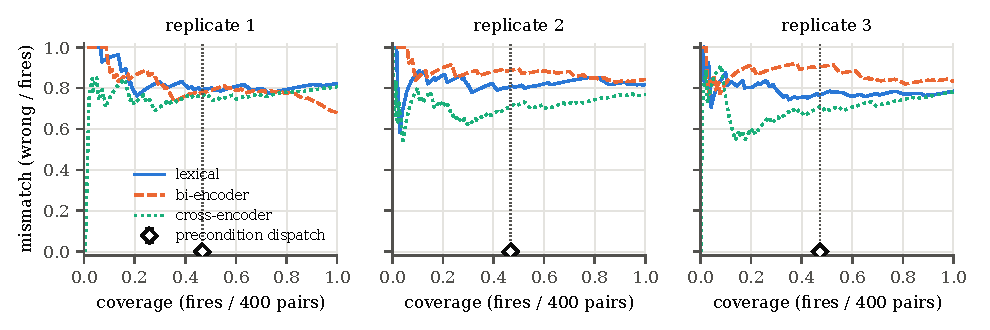
\includegraphics[width=\linewidth]{figures/curves.pdf}
\caption{Mismatch against coverage on the eval block, per replicate. Each text scorer's curve
holds every operating point its threshold sweep can reach; the diamond is precondition
dispatch, with its 95\% Wilson interval, and the dotted line its coverage, where arm 2 is
matched.}
\label{fig:curves}
\end{figure}

\begin{table}[t]
\centering
\caption{Fires and wrong fires at matched coverage on the eval block.}
\label{tab:synthetic}
\small
\begin{tabular}{lccc}
\toprule
& replicate 1 & replicate 2 & replicate 3 \\
\midrule
precondition dispatch & 187, \textbf{0} & 187, \textbf{0} & 189, \textbf{0} \\
lexical similarity & 187, 148 & 185, 149 & 187, 143 \\
bi-encoder similarity & 185, 143 & 189, 168 & 187, 169 \\
cross-encoder similarity & 186, 142 & 187, 133 & 189, 134 \\
\midrule
state reader (one fit) & \multicolumn{3}{c}{190, 0} \\
\bottomrule
\end{tabular}
\end{table}

\paragraph{Result.}
Precondition dispatch mis-fired on none of its 563 fires (Table~\ref{tab:synthetic},
Figure~\ref{fig:curves}). The text scorers mis-fired on 71--90\% of theirs at the same coverage,
about five times $\delta^\ast$. The flatness of the curves in Figure~\ref{fig:curves} is the
identity of Section~\ref{sec:identity} at work: thresholding a score that carries no information
about the state removes fires without making the remainder more right.

\paragraph{Why this is not the result.}
Each pair's acceptable set is a rule over the observed state, and the rule is ours. The state
reader fired on 190 of the 400 pairs, none wrongly, and on the held-out block it fired on 200,
none wrongly, where precondition dispatch had 13, 8 and 21 mis-fires. So the table supports only
the weaker claim that a dispatcher that reads the state beats one that does not.

\paragraph{Held-out states, and a mechanism.}
On the held-out block four sources carried: one mis-fire in 480 fires. The lock-file source, which
moves the conflicted file to a nested path, a path with a space, a non-ASCII name or a dotfile,
did not: 41 of 101 fires were wrong, every one on a path with a space or a non-ASCII character.
The cause is a class of probe. Git quotes such paths in its default output, so a probe that
reads a path list without \code{-z} and compares, greps or splits it finds nothing. Each such
probe was an \emph{absence} check, so finding nothing meant it held, and the program fired. Two
of the mis-firing programs were \code{diverged}'s \code{discard}, which on a lock-file state
throws the local dependency change away. Admission passed them because no admit-seed path needed
quoting. Reading the libraries found at least 16 such probes in 10 of their 40 admitted programs.
The failure is general: an absence check fails \emph{open} when its reading of the state breaks.

\paragraph{What a fire does.}
Replaying each of arm 3's 563 fires on a fresh build of its state fixed 536. The other 27, all in
replicate 3, came from two programs that pass their own postconditions while the fault's checker
refuses what they leave. Arm 2's 318 fires on fault-free states changed nothing, and on a fault's
state 147 of its 241 fires fixed it. No replay of either arm lost a recorded commit.

\section{A pre-registered test on real lock-file merges}
\label{sec:real}

\subsection{Registration}

Before any case was mined we committed a registration whose SHA-256 is pinned in the code; the
measurement refuses to run unless the document is present, committed and unchanged. It fixes the
hypotheses, the ordered repository list, the case and label definitions, the analysis and the
decision rules. A pilot of 44 merges motivated one amendment, committed before the confirmatory
data was mined, and tests nothing.

\paragraph{Hypotheses.}
Rule 2: precondition dispatch rarely mis-fires, meaning the Wilson lower bound of its mismatch is
at most 0.10. H1: at matched coverage it mis-fires less than lexical similarity. H2: it
mis-fires less than the state reader. H3, added by the amendment: it fires less often than the
state reader on conflicts no resolution can express. Only H2 could license a sentence saying
that executing checks, rather than reading the state, is what wins.

\subsection{Cases and labels}

A \emph{conflicted case} is a two-parent merge whose sides both changed a lock file and whose
\code{git merge-tree} conflicts in it. A \emph{clean case} changed a lock file on both sides and
merged cleanly; per repository, as many clean cases as conflicted, the most recent first.
Criss-cross merges and submodule or binary conflicts are excluded and counted. The state is a
checkout of the first parent, tracking upstream's default branch at the second parent.

For each conflicted lock file the base's, parents' and merge's versions are read as multisets of
lines, $B$, $L$, $U$ and $M$. \code{take\_upstream} produces $U+(L-B)$ and \code{keep\_local}
produces $L+(U-B)$. A resolution is acceptable if what it produces equals $M$ for every conflicted
lock file, and only lock files conflicted. \code{merge} is acceptable on a clean case whose
committed tree equals the tree \code{git merge-tree} writes. A conflicted case with an empty
acceptable set is \emph{inexpressible}.

Sixteen of the 18 listed repositories were mined, in order, until the target of 247 cases from at
least 8 repositories was met; five yielded no case. The set has 274 cases from 11 repositories,
161 conflicted and 113 clean, and three exclusions. No repository exceeds the registered cap.

\subsection{Results}

\begin{table}[t]
\centering
\caption{Real lock-file merges, by library. Mismatch is wrong over fired, with its 95\% Wilson
interval; differences carry 95\% bootstrap intervals clustered by repository.}
\label{tab:real}
\small
\begin{tabularx}{\linewidth}{Xccc}
\toprule
& library 1 & library 2 & library 3 \\
\midrule
precondition dispatch & 62/150 [.34,.49] & 10/122 [.05,.14] & 132/244 [.48,.60] \\
\quad right on clean merges & 87 of 113 & 112 of 113 & 112 of 113 \\
\quad right on conflicts & 1 of 37 & 0 of 9 & 0 of 131 \\
lexical similarity, matched & 140/150 & 122/122 & 239/244 \\
state reader & 159/160 & 159/160 & 159/160 \\
\midrule
H1 = lexical $-$ arm 3 & $+$.52 [.36,.69] & $+$.92 [.81,.98] & $+$.44 [.28,.56] \\
H2 = state reader $-$ arm 3 & $+$.58 [.43,.74] & $+$.91 [.80,.98] & $+$.45 [.28,.59] \\
H3, fire rates on inexpressible & $+$.77 [.61,.89] & $+$.94 [.85,.99] & $+$.18 [.05,.35] \\
\bottomrule
\end{tabularx}
\end{table}

\paragraph{Decisions, as registered.}
Rule 2 is \textbf{falsified}: the lower bound of precondition dispatch's mismatch is 0.338 and
0.478 in two of three libraries. H1, H2 and H3 are supported in every library
(Table~\ref{tab:real}).

\paragraph{Where the margins come from.}
Almost no conflict is expressible. Maintainers regenerated the lock file on 79 of the 161
conflicts, did something else on 48, took the local side on 20 and upstream's on 12; only 2
matched what \code{take\_upstream} produces. The intent's own rule disagrees with the maintainer on
37 conflicted cases. Precondition dispatch's right fires are \code{merge} on clean merges, fired
from another intent's programs, which the registration counts as right. The registered state
reader decides with the lock-file intent's own tree, so it can never fire \code{merge}. H2
therefore compares fires on mostly clean cases with fires on conflicted ones; wherever both
dispatchers fired, both were wrong, and McNemar's test on joint fires has no discordant pair in
any library. We read H2 as a flaw in the registered control's scope, not as evidence for
executing preconditions. H1's McNemar counts, 66/3, 89/0 and 105/0 discordant pairs, show that
its margin also comes mostly from clean merges, where arm 2's top candidate is \code{merge} on 9,
0 and 0 of the 113.

\begin{figure}[t]
\centering
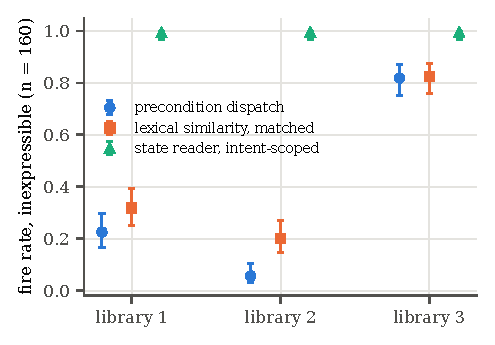
\includegraphics[width=0.55\linewidth]{figures/refusal.pdf}
\caption{Fire rate on stage B's 160 inexpressible conflicts, where any fire is wrong, with 95\%
Wilson intervals. Lexical similarity is read at its operating point matched to precondition
dispatch.}
\label{fig:refusal}
\end{figure}

\paragraph{Exploratory: a reader with the same scope.}
After seeing the data, we gave the state reader arm 3's scope: it fires the most probable
resolution any intent's tree predicts. This tests nothing. It was right on 110 of the 112 clean
merges it fired on, as often as precondition dispatch, and fired on all 161 conflicts, none
rightly. Its \code{merge} comes from a tree whose rule refuses a conflicting sync, but only 4 of
its 56 training states conflict, so it never learned to refuse. The compiled \code{merge}
programs instead run a probe that tries the merge and refuse when it would conflict. In this data,
refusal is the one place where executing a check differed from reading the state, and it varied
by library (Figure~\ref{fig:refusal}).

\subsection{Verification}

A script importing nothing from the project recomputes every count, matched point, point
estimate and rule-2 bound from the released files exactly; with its own seed, its bootstrap
intervals fall within 0.01 of the registered ones. A second script re-fetched five repositories
(55 cases, 20\%) at their pinned tips and re-derived every label from git alone. All 55 agree.

\section{Are the graders right?}
\label{sec:graders}

Every figure depends on graders written in this project: each fault's \code{check}, and the
\code{recorded\_state\_intact} family that refuses a resolution destroying recorded work. We
mutated them one small change at a time and ran the 15 test files that grade, taking 88.7\,s per
clean run, with \code{-x}. A mutant every test still passes \emph{survived}: no test exercises the
clause it changed. Table~\ref{tab:mutation} gives the outcomes by operator. A mutant inside a
verdict's message (an f-string or a \code{detail=} argument) can change what a verdict says but
never whether it passes, and is reported apart; that classification is syntactic.

\begin{table}[t]
\centering
\caption{Mutants of the graders by operator. The score is killed over mutants that can change a
verdict: 133 of 141, 0.943.}
\label{tab:mutation}
\small
\begin{tabular}{lrrrr}
\toprule
operator & mutants & killed & survived & message only \\
\midrule
comparison flipped (\code{==}, \code{is}, \code{in} and negations) & 42 & 42 & 0 & 0 \\
\code{not} removed & 15 & 15 & 0 & 0 \\
boolean constant swapped & 56 & 51 & \textbf{5} & 0 \\
integer moved by one & 48 & 20 & \textbf{2} & 26 \\
\code{and}/\code{or} swapped & 10 & 5 & \textbf{1} & 4 \\
\midrule
total & 171 & 133 & 8 & 30 \\
\bottomrule
\end{tabular}
\end{table}

\paragraph{The five real gaps.}
All five survivors among the boolean swaps turn a failure into a pass, \code{ok=False} into
\code{True}:
\begin{itemize}
  \item \code{config\_renamed}, three clauses: the renamed key set to a different value than the
  one it must keep; another setting in the target file changed; and, in the state where the old
  key lives only in a git-ignored override, the already-current settings file edited.
  \item \code{submodule\_moved}, two clauses: \code{repin} accepted after upstream no longer
  records the submodule at all; and an injected state the checker does not know.
\end{itemize}
Each now has a test written against it, and each mutant, applied alone, fails that test while the
unmutated grader passes it. None of these clauses was reached by any state the benchmark builds:
they guard against fixes an agent might make, or states the harness never injects. So no reported
figure was graded by a broken clause, but an agent's wrong fix could have been graded right.

\paragraph{The three equivalent survivors.}
\begin{itemize}
  \item \code{config\_renamed}: \code{values[0]} became \code{values[-1]}. The line before
  requires \code{len(values) == 1}, so the two name the same element.
  \item \code{lockfile\_conflict}: \code{splitlines()[0]} became \code{[-1]}. The verdict is
  already \code{False} once any conflict marker remains; the index only picks which marker line
  the message quotes. It is message-only in effect, but the index sits in an assignment outside
  the \code{detail=} argument, so the syntactic rule could not see that.
  \item \code{submodule\_moved}: \code{if in\_tree and in\_modules} became \code{or}. The
  branches only choose the wording of a failure, and every branch fails.
\end{itemize}

\paragraph{What this does and does not show.}
With the five closed and the three argued equivalent, no clause that can change a verdict is left
unexercised by these operators. That is not every defect: a wrong constant, a missing clause or a
wrong rule is not a mutation the runner makes, and a grader that accepts too much is caught only
if some test presents a wrong resolution. Property-based tests check two graders on 300
generated states each, with no failure \cite{maciver2019hypothesis}. Agreement with human judges
has not been measured.

\section{The registered follow-up study, and its power}
\label{sec:power}

\subsection{Design}

The exploratory finding is a hypothesis. We registered a second study before any of its data
exists. It treats builds as a population: 10 builds in each of two configurations, build $b$
permuting the order of the admit plan with seed $b$. Configuration~0 is the current gate.
Configuration~R also admits a program only if its preconditions refuse every state of a frozen set
$R$ of up to 40 real inexpressible conflicts from four admission repositories. Control-0 is the
library-scoped state reader fitted on the 56 states; Control-R is the same reader also fitted on
$R$, labelled ``fire nothing''. With $f(\cdot)$ the fire rate on the evaluation set's
inexpressible conflicts:

\begin{itemize}
  \item H1 (primary): $\overline{f(\text{Control-R}) - f(b)}_{b\in R} > 0$, the only comparison
  in which both sides have the same refusal evidence;
  \item H2: the same for configuration 0 against Control-0;
  \item H3: $\bar f_0 - \bar f_R > 0$;
  \item H4 (guard): configuration R's right-fire rate on clean cases is not lower than 0's by
  more than 0.10.
\end{itemize}

Each interval is a 95\% two-level bootstrap: each of 2000 resamples draws the evaluation
repositories with replacement, then each configuration's builds with replacement. H1--H3 are
supported if the lower bound is above 0, and H4 holds if it is above $-0.10$. Evaluation cases
come from 12 repositories no earlier stage touched, mined only after all 20 libraries are frozen,
until there are 100 inexpressible conflicts and 60 clean cases from at least 6 repositories. The
code implementing all of this is reviewed before any of $R$ is mined. Six choices the registration
leaves open, such as the per-repository cap and whether an $R$ refusal gets the one revision
other refusals get, were decided and recorded before any data.

\subsection{A Monte Carlo power analysis}

The registration states its power from a back-of-envelope interval half-width. We instead
simulate the study under explicit assumptions and apply its registered decision rules.

\paragraph{The generating model.}
Case $i$ in repository $r$ is fired on by build $b$ with probability
$\operatorname{logistic}(a_b+u_r+v_i)$, with $a_b\sim N(\operatorname{logit} m, s_b)$, $u_r\sim
N(0,s_r)$ and $v_i\sim N(0,s_c)$. A control is one dispatcher, so it is one draw. The build
spread $s_b=2.19$ is calibrated on study 1, whose three libraries fired on 22.5\%, 5.6\% and
81.9\% of the inexpressible conflicts; their logits have that standard deviation. The clean-case
build spread, calibrated the same way on study 1's right rates of 87, 112 and 112 of 113, is
2.03. The repository and case spreads have no anchor and are varied. The evaluation set has 100
inexpressible conflicts from 7 repositories (30, 25, 15, 10, 8, 7 and 5) and 60 clean cases in
the same proportions. Every reported rate is the realised mean, computed numerically, since a
centre on the logit scale is not a mean.

\paragraph{The bootstrap, validated.}
The registered bootstrap is pure Python and too slow for thousands of simulated studies, so the
analysis uses a vectorised copy. On three simulated studies it gives point estimates identical to
the registered code's and interval ends within 0.03, the difference being only which resamples
each draws. Each power figure is the share of 400 simulated studies, and each false-positive rate
the share of 2000, in which the hypothesis is supported.

\begin{figure}[t]
\centering
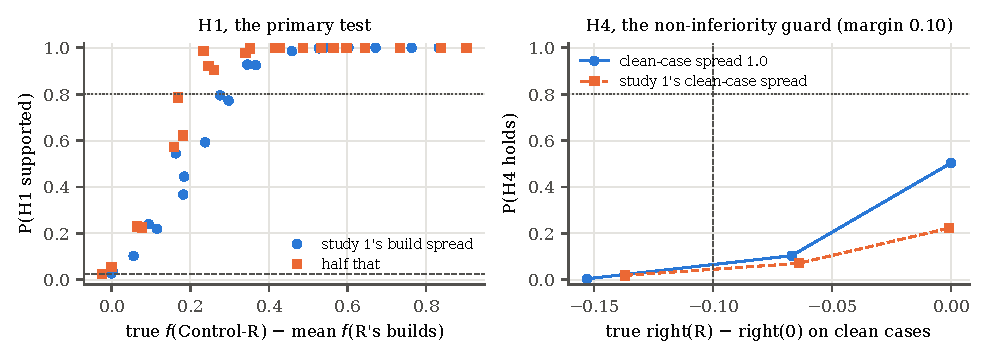
\includegraphics[width=\linewidth]{figures/power.pdf}
\caption{Power of the registered tests. Left: H1 against the true difference, over scenarios of
Control-R's fire rate and configuration R's builds, at study 1's build spread and half of it.
Right: the probability that H4 holds against the true difference in clean-case right rates,
averaged over the H3 scenarios; the dashed line is the margin.}
\label{fig:power}
\end{figure}

\begin{table}[t]
\centering
\caption{Simulated operating characteristics of the registered tests (one-sided, nominal 2.5\%).
Differences are realised means.}
\label{tab:power}
\small
\begin{tabularx}{\linewidth}{Xcc}
\toprule
scenario & true difference & P(supported) \\
\midrule
H1, study 1's build spread, Control-R at 0.50 & 0.28 & 0.80 \\
H1, study 1's build spread, Control-R at 0.50 & 0.18 & 0.45 \\
H1, half the build spread, Control-R at 0.50 & 0.25 & 0.92 \\
H1, no difference (2000 studies), two spreads & 0 & 0.032, 0.035 \\
H2, Control-0 at 0.99 as in study 1 & 0.56 & 1.00 \\
H3, study 1's build spread & 0.27 & 0.60--0.70 \\
H3, half the build spread & 0.25 & 0.91--0.95 \\
H3, no difference (2000 studies), two spreads & 0 & 0.038, 0.028 \\
H4 holds, no true cost, clean-case spread 1.0 & 0 & 0.47--0.53 \\
H4 holds, no true cost, study 1's clean-case spread & 0 & 0.19--0.26 \\
H4 holds, true cost 0.065, inside the margin & $-$0.065 & 0.06--0.11 \\
\bottomrule
\end{tabularx}
\end{table}

\paragraph{What it shows.}
Table~\ref{tab:power} and Figure~\ref{fig:power} give the results.

\begin{itemize}
  \item \textbf{The primary test's stated power holds.} The registration says H1 can detect a
  difference of about 0.3. At study 1's build spread, a true difference of 0.28 is detected with
  probability 0.80. Calmer builds lower that to about 0.25. H3's stated sensitivity of about 0.4
  is consistent too: 0.27 is detected with probability 0.60--0.70.
  \item \textbf{The false-positive rates are a little above nominal}: 2.8--3.8\% against 2.5\%.
  This is the percentile bootstrap's known slight anti-conservatism with only ten builds per
  group. It is small, and we report it rather than adjust the registered rule.
  \item \textbf{Results are insensitive to the unanchored spreads.} Setting the repository and
  case spreads to 0, or the repository spread to 1.0, or the case spread to 1.5, moves H1's power
  in the $s_b=2.19$, difference-0.28 scenario between 0.73 and 0.80.
  \item \textbf{The non-inferiority guard cannot do its job.} With no true cost at all, H4 holds
  in about half the simulated studies with a clean-case build spread of 1.0, and in only a fifth
  to a quarter with study 1's spread. The reason is arithmetic. Under the model, the builds' right
  rates on the 60 clean cases have a standard deviation $\sigma$ of about 0.10 at the calmer
  spread and 0.22 at study 1's. The difference of two means of ten builds then has standard error
  $\sqrt{2}\,\sigma/\sqrt{10}$, 0.045 or 0.097, so the 95\% interval's half-width from builds
  alone is 0.09 or 0.19, before resampling repositories widens it further. With a true difference
  of zero, the lower bound clears $-0.10$ only when the half-width happens to fall below the
  margin: about half the time at the calmer spread, and rarely at study 1's. More clean cases
  cannot fix that; only more builds or a calmer build process could.
\end{itemize}

\paragraph{Consequence for the decision rules.}
Rule 5 reads ``H3 supported and H4 fails'' as ``refusal-tested admission buys declining at the
cost of clean merges''. Under the simulation, given H3 is supported and there is no true cost,
H4 fails most of the time, so the registered sentence would usually be false. This is a design
flaw found before any data exists, and the registration permits an amendment then. We propose
that a failed H4 be reported as ``non-inferiority not shown'', with the H4 interval, and that
only an interval lying wholly below $-0.10$ be read as a cost. Whether to adopt this is the
repository owner's decision, recorded in the registration before the study runs.

\section{Comparison with executability gating and retrieval-risk measurement}
\label{sec:comparison}

\begin{table}[t]
\centering
\caption{Three ways to keep an agent from running the wrong skill.}
\label{tab:comparison}
\small
\begin{tabularx}{\linewidth}{lXXX}
\toprule
& executability gate \cite{wix2026gating} & retrieval risk \cite{ding2026rightfamily} & this work \\
\midrule
decides & which candidates the model may see & which skills retrieval exposes & which program runs \\
checks & hand-written exit predicates on authoritative account state & the query's text against each skill's contract & LLM-compiled probes on the live repository \\
place & after semantic recall & retrieval itself & alone, or after retrieval (hybrid) \\
guarantee & one-sided: a removed skill cannot run & none: exposure is measured & all preconditions held when it fired \\
measures & counterfactual mis-selection; context reduction & harmful-sibling rate at $K$ & mismatch at matched coverage \\
graded by & production state & benchmark contracts & own rules; maintainers' commits \\
\bottomrule
\end{tabularx}
\end{table}

\paragraph{The executability gate \cite{wix2026gating}.}
In a deployed customer-care agent covering a ten-skill domain family, a recall-oriented semantic
matcher proposes candidate skills without looking at account state. A deterministic gate then
removes every candidate whose hard exit predicates hold on authoritative state, before its
description reaches the model. The guarantee is one-sided: passing the gate means no represented
exit condition holds, not that the user wants the skill. In a counterfactual replay of 1,000
conversations without the gate, the model selected a skill production would have blocked in 78,
7.8\%; matching plus gating cut skill-description context by 90.5\% against exposing all ten
descriptions. The authors claim no downstream tool-execution or customer-outcome effect.

Three points of contact follow.

\begin{enumerate}
  \item \textbf{The cascade.} Their architecture is recall then gate. Our hybrid arm is exactly
  that shape: retrieve the top $k$ by text, then fire the first whose preconditions hold. On our
  libraries the hybrid never mis-fired and never fired more often than the gate alone, and by
  construction it cannot: its fires are a subset of arm 3's. Capping $k$ only dropped correct
  fires: at $k=1$, 56--76 of arm 3's 187--189. But as the \emph{order} in which to try programs,
  stopping at the first that holds, text cut the checks evaluated by 29--37\% with identical
  decisions, against 20\% for trying the most specific program first. So on our states retrieval
  before a gate is an efficiency device, not an accuracy one. That is consistent with their
  reported gains being in context, not in correctness.
  \item \textbf{One-sided checks fail open.} Their exit predicates block. Our held-out failure
  shows how blocking checks break: an absence check whose reading of the state silently fails
  reports ``absent'' and lets the program through. Hand-written predicates over a typed account
  API are less exposed than LLM-written shell probes over git's quoted output, but the failure
  mode is the same, and it is invisible to a funnel metric.
  \item \textbf{What neither measures.} Their counterfactual measures the model's selection
  error when the gate is removed, and ours measures the dispatcher's own error at matched
  coverage. Neither alone says how often a gated system runs the wrong skill on states nobody
  anticipated. Our real-merge study is one answer for one domain, and it was not comforting.
\end{enumerate}

\paragraph{The retrieval-risk benchmark \cite{ding2026rightfamily}.}
Each unit pairs a helpful skill with a query-specific risky sibling from the same capability
family, differing on an execution-controlling contract: a required resource, a precondition, a
procedure or an artifact. The metric is the harmful-sibling rate among the top $K$ retrieved,
HSR@$K$. The paper has changed title and size across versions; in its second version, public
retrievers had HSR@3 of 0.346--0.372 and a resolver that uses the contracts 0.007.

\begin{enumerate}
  \item \textbf{The same object, seen from two sides.} Their risky sibling is our same-intent
  negative class: a program for \code{take\_upstream} on a state where \code{keep\_local} is
  right. They measure whether retrieval \emph{exposes} it; we measure whether a dispatcher
  \emph{fires} it, at matched coverage, and require admission to refuse it.
  \item \textbf{Why our text scorers do so much worse.} Our text arms are wrong on 71--90\% of
  fires, far above their retrievers' HSR@3. The difference is not scorer quality. Their queries
  state the contract, so a contract-aware resolver can nearly eliminate exposure from text.
  Ours, on the uninformed channel, carry no information about the state by construction
  (Proposition~1), so no text scorer can separate siblings. The two results bracket text-based
  dispatch: it can work when the request states what distinguishes the right skill, and cannot
  when only the environment does.
  \item \textbf{What both leave out.} Both assume a right skill exists among the candidates. On
  real lock-file conflicts it almost never did, 1 of 161. There the right action is to refuse,
  and the measure is how often a dispatcher declines. A one-sided gate refuses only what its
  predicates anticipated; study 2 asks whether admission can select for refusal of what was not.
\end{enumerate}

\section{Threats to validity}

\begin{itemize}
  \item \textbf{Construct.} Mis-fire is judged against an acceptable set. On real merges, a
  resolution that differs from the maintainer's commit counts as wrong even if it would build.
  The external oracles, the ecosystem's lock-file tools and the projects' own tests, are not
  built.
  \item \textbf{Internal.} The libraries come from one LLM at temperature 0, three builds, which
  differ widely. The registered control's scope was a design flaw (Section~\ref{sec:real}). The
  power analysis rests on a generating model whose build spread is calibrated on three builds.
  \item \textbf{External.} One family of faults, and on real data only lock-file merges from 11
  repositories. Nothing is measured at episode level: cost, the misses an agent would then
  solve, and online learning were not run at scale.
  \item \textbf{Text scorers.} Only local scorers were compared. An LLM judge reading the state is
  implemented and registered, and has not been run.
  \item \textbf{Author.} One author built the apparatus, wrote the graders and ran the analyses.
  The pre-registrations, the independent recomputation and the mutation tests mitigate this;
  they are not independent review.
\end{itemize}

\section{Conclusion}

On states we built and labelled, executable-precondition dispatch never mis-fired, but neither
did a classifier that only reads the state, and the request channel was built to carry nothing a
text scorer could use. On real lock-file merges, graded by what maintainers committed, the claim
that precondition dispatch rarely mis-fires was falsified. What survived is narrow: it fires
\code{merge} on clean merges where text similarity does not, and some libraries refuse conflicts
nothing can resolve. The follow-up study that tests refusal is registered; simulating it through
its own decision rules confirmed its primary test and exposed a guard that cannot do its job,
before any of its data exists. The broader lesson is about evaluation: an error rate measured
against one's own labels says little until the same dispatcher faces states and labels someone
else made, and a registered design deserves the same scrutiny before its data as its results
receive after.

\section*{Data and code availability}

The apparatus, the three libraries, every result file, both registrations and the verification
scripts are at \url{https://github.com/Shyboy0499/precondition-library}. The figures and tables of
Sections~\ref{sec:synthetic}--\ref{sec:graders} come from committed result files; the power
analysis and every figure are regenerated by \code{paper/analysis/power.py} and
\code{paper/analysis/figures.py}. Only commit SHAs and derived labels from mined repositories are
released, never their content.

\section*{Use of generative AI}

The software, analyses and text of this report were produced with substantial assistance from an
AI coding assistant (Claude Code, Anthropic), directed and reviewed by the author. The libraries
under study were compiled by a separate commercial LLM, as Section~\ref{sec:synthetic} describes.
The author takes full responsibility for the contents.

\begin{thebibliography}{99}

\bibitem{cai2024latm}
T.~Cai, X.~Wang, T.~Ma, X.~Chen and D.~Zhou.
\newblock Large language models as tool makers.
\newblock In \emph{International Conference on Learning Representations (ICLR)}, 2024.
\newblock arXiv:2305.17126.

\bibitem{chen2026skilldroid}
Q.~Chen, A.~Bellucci, Z.~Sun and G.~Jacucci.
\newblock {SkillDroid}: Compile once, reuse forever.
\newblock arXiv:2604.14872, 2026.

\bibitem{ding2026rightfamily}
J.~Ding, H.~Ji, M.~Liu and T.~Duan.
\newblock Right family, wrong skill: Evaluating risk exposure in agent skill retrieval.
\newblock arXiv:2606.10388v4, 2026. Earlier versions were titled \emph{SkillResolve-Bench}; the
figures quoted here are from version 2.

\bibitem{fikes1972macrops}
R.~E. Fikes, P.~E. Hart and N.~J. Nilsson.
\newblock Learning and executing generalized robot plans.
\newblock \emph{Artificial Intelligence}, 3:251--288, 1972.

\bibitem{jaber2026auto}
J.~Jaber and O.~Jaber.
\newblock Auto: The {AGI} compiler.
\newblock arXiv:2607.04542, 2026.

\bibitem{jia2011mutation}
Y.~Jia and M.~Harman.
\newblock An analysis and survey of the development of mutation testing.
\newblock \emph{IEEE Transactions on Software Engineering}, 37(5):649--678, 2011.

\bibitem{laird1986chunking}
J.~E. Laird, P.~S. Rosenbloom and A.~Newell.
\newblock Chunking in {Soar}: The anatomy of a general learning mechanism.
\newblock \emph{Machine Learning}, 1(1):11--46, 1986.

\bibitem{li2026preact}
B.~Li.
\newblock {PreAct}: Computer-using agents that get faster on repeated tasks.
\newblock arXiv:2606.17929, 2026.

\bibitem{maciver2019hypothesis}
D.~R. MacIver, Z.~Hatfield-Dodds and many other contributors.
\newblock Hypothesis: A new approach to property-based testing.
\newblock \emph{Journal of Open Source Software}, 4(43):1891, 2019.

\bibitem{nosek2018preregistration}
B.~A. Nosek, C.~R. Ebersole, A.~C. DeHaven and D.~T. Mellor.
\newblock The preregistration revolution.
\newblock \emph{Proceedings of the National Academy of Sciences}, 115(11):2600--2606, 2018.

\bibitem{reimers2019sbert}
N.~Reimers and I.~Gurevych.
\newblock Sentence-{BERT}: Sentence embeddings using {Siamese} {BERT}-networks.
\newblock In \emph{Proceedings of EMNLP-IJCNLP}, 2019.

\bibitem{smyth1998adaptation}
B.~Smyth and M.~T. Keane.
\newblock Adaptation-guided retrieval: Questioning the similarity assumption in reasoning.
\newblock \emph{Artificial Intelligence}, 102(2):249--293, 1998.

\bibitem{sutton1999options}
R.~S. Sutton, D.~Precup and S.~Singh.
\newblock Between {MDPs} and semi-{MDPs}: A framework for temporal abstraction in reinforcement
learning.
\newblock \emph{Artificial Intelligence}, 112(1--2):181--211, 1999.

\bibitem{wang2023voyager}
G.~Wang, Y.~Xie, Y.~Jiang, A.~Mandlekar, C.~Xiao, Y.~Zhu, L.~Fan and A.~Anandkumar.
\newblock Voyager: An open-ended embodied agent with large language models.
\newblock arXiv:2305.16291, 2023.

\bibitem{wilson1927}
E.~B. Wilson.
\newblock Probable inference, the law of succession, and statistical inference.
\newblock \emph{Journal of the American Statistical Association}, 22(158):209--212, 1927.

\bibitem{wix2026gating}
O.~Ashkenazi, V.~Kloz and M.~Ulianchenko.
\newblock Don't offer what can't be done: Deterministic executability gating for {LLM} skill
selection at scale.
\newblock arXiv:2608.01050, 2026.

\end{thebibliography}

\end{document}
